\documentclass[a4paper, 11pt]{article}
\usepackage[left=1.5cm,text={17cm, 24cm},top=3.0cm]{geometry}
\usepackage[utf8x]{inputenc}
\usepackage[czech]{babel}
\usepackage[T1]{fontenc}
\usepackage{times}
\usepackage{graphics}
\usepackage[czech,ruled,linesnumbered,noline]{algorithm2e}
\usepackage{multirow}

\begin{document}

\thispagestyle{empty}
\begin{center}
	\Huge
	\textsc{Vysoké učení technické v~Brně\\\vspace{-0.10cm}\huge{Fakulta informačních technologií}}\\
	\LARGE
	\vspace{\stretch{0.382}}
		
		\LARGE{Typografie a~publikování \,--\ 3. projekt}\\\vspace{-0.05cm}\Huge{Tabulky a obrázky}
	
	\vspace{\stretch{0.618}}
	{\Large 5. dubna 2015 \hfill Daniel Dušek }
\end{center}

\newpage


\section{Úvodní strana}
Název práce umístěte do zlatého řezu a nezapomeňte uvést dnešní datum a vaše jméno a příjmení

\section{Tabulky}
Pro sázení tabulek můžeme použít buď prostředí \verb|tabbing| nebo prostředí \verb|tabular|.
	
	\subsection{Prostředí \texttt{tabbing}}
	Při použití \verb|tabbing| vypadá tabulka následovně:

	\begin{tabbing}

	\textbf{Ovoce} \quad \hspace{1.2cm} \= \textbf{Cena} \hspace{0.3cm} \= \textbf{Množství}- \\
	Jablka \> 25,90 \> 3~kg \\
	Hrušky \> 27.40 \> 2.5~kg \\
	Vodní~melouny \> 35,- \> 1~kus \\

	\end{tabbing}

Toto prostředí se dá také použít pro sázení algoritmů, ovšem vhodnější je použít prostředí algorithm nebo algorithm2e (viz sekce 3).

\subsection{Prostedí \texttt{tabular}}

Další možností, jak vytvořit tabulku, je použít prostředí \texttt{tabular}. Tabulky pak budou vypadat takto\footnotemark[1]:

\begin{table}[h]

	\begin{center}
	\catcode `\-=12

	\begin{tabular}{|l|r|r|}
	\hline

		\hline
		& \multicolumn{2}{|c|}{\textbf{Cena}} \\
		\cline{2-3}
		
		\textbf{Měna} & \textbf{nákup} & \textbf{prodej} \\
		\hline
		EUR & 27,34 & 27,42 \\
		GBP & 33,09 & 33,21 \\
		USD & 19,87 & 19,95 \\
		\hline
	\end{tabular}

	\caption{Tabulka kurzů k dnešnímu dni}
	\label{tabulka1}


	\end{center}


\end{table}

\begin{table}[ht]
\begin{center}
\catcode `\-=12
	\begin{tabular}{|c|c|}
			\hline
			$A$ & $\neg A$ \\
			\hline
			\textbf{P} & N \\
			\hline
			\textbf{O} & O \\
			\hline
			\textbf{X} & X \\
			\hline
			\textbf{N} & P \\
			\hline
	\end{tabular}
	\begin{tabular}{|c|c|c|c|c|c|}
		\hline

			\multicolumn{2}{|c|}{\multirow{2}{*}{$A \wedge B$}} & \multicolumn{4}{|c|}{$B$} \\
			\cline{3-6}

			\multicolumn{2}{|c|}{} & \textbf{P} & \textbf{O} & \textbf{X} & \textbf{N} \\ 
			\hline
			\multirow{4}{*}{A} & \textbf{P} & P & O & X & N \\ 
			\cline{2-6}
			& \textbf{O} & O & O & N & N \\
			\cline{2-6}
			 & \textbf{X} & X & N & X & N \\
			\cline{2-6}
			& \textbf{N} & N & N & N & N \\


			\hline

		\hline
	\end{tabular}
	\begin{tabular}{|c|c|c|c|c|c|}
		\hline

			\multicolumn{2}{|c|}{\multirow{2}{*}{$A \vee B$}} & \multicolumn{4}{|c|}{$B$} \\
			\cline{3-6}

			\multicolumn{2}{|c|}{} & \textbf{P} & \textbf{O} & \textbf{X} & \textbf{N} \\ 
			\hline
			\multirow{4}{*}{A} & \textbf{P} & P & P & P & P \\ 
			\cline{2-6}
			& \textbf{O} & P & O & P & O \\
			\cline{2-6}
			 & \textbf{X} & P & P & X & X \\
			\cline{2-6}
			& \textbf{N} & P & O & X & N \\


			\hline

		\hline
	\end{tabular}
	\begin{tabular}{|c|c|c|c|c|c|}
		\hline

			\multicolumn{2}{|c|}{\multirow{2}{*}{$A \rightarrow B$}} & \multicolumn{4}{|c|}{$B$} \\
			\cline{3-6}

			\multicolumn{2}{|c|}{} & \textbf{P} & \textbf{O} & \textbf{X} & \textbf{N} \\ 
			\hline
			\multirow{4}{*}{A} & \textbf{P} & P & O & X & N \\ 
			\cline{2-6}
			& \textbf{O} & P & O & P & 0 \\
			\cline{2-6}
			 & \textbf{X} & P & P & X & X \\
			\cline{2-6}
			& \textbf{N} & P & P & P & P \\


			\hline

		\hline
	\end{tabular}
\end{center}
	\caption{Protože Kleeneho trojhodnotová logika už je \uv{zastaralá}, uvádíme si zde příklad čtyřhodnotové logiky}
	\label{tabulka2}

\end{table}



\footnotetext[1]{Kdyby byl problém s \texttt{cline}, zkuse se podívat třeba sem: http://www.abclinuxu.cz/text/poradna/show/325037.}


\newpage

\section{Algoritmy}
Pokud budeme chtít vysázet algoritmus, můžeme použít prostředí \texttt{algorithm}\footnotemark[2] nebo \texttt{algorithm2e}\footnotemark[3]. Příklad použití prostředí \texttt{algorith2e} viz Algoritmus 1.

\begin{algorithm}[H]
\caption{\sc{FastSLAM}}

	\SetKwInOut{Input}{Input}
	\SetKwInOut{Output}{Output}

	\Input{$(X_{t-1}, u_t, z_t)$}
	\Output{$X_t$}

	\BlankLine

	$\overline{X_t} = X_t = 0$\\
	\For{$k=1$ \textnormal{to} $M$ }
	{

		$x_t^{[k]} = $ \emph{sample\_motion\_model $(u_t,x_{t-1}^{[k]})$} \\
		$w_t^{[k]} = $ \emph{measurement\_model} $(z_t,x_t^{[k]},m_{t-1})$ \\
		$m_t^{[k]} = $ \emph{updated\_occupancy\_grid} $z_t,x_t^{[k]},m_{t-1}^{[k]})$ \\
		$\overline{X_t} = \overline{X_t} + \langle x_x^{[m]}, w_t^{m} \rangle$

	}
	\For{$k=1$ \textnormal{to} $M$}
	{
		\textnormal{draw} $i$ \textnormal{with probability} $\approx w_t^{[i]}$ \\
		\textnormal{add} $\langle x_x^{[k]}, m_t^{[k]}$ \textnormal{to} $X_t$
	}
	\Return{$X_t$}

\label{algoritmus1}
\end{algorithm}

\footnotetext[2]{Pro nápovědu, jak zacházet s prostředím algorithm, můžete zkusit tuhle stránku:\\ http://ftp.cstug.cz/pub/text/CTAN/macros/latex/contrib/algorithms/algorithms.pdf.}
\footnotetext[3]{Pro \texttt{algorithm2e} zase tuhle: http://ftp.cstug.cz/pub/text/CTAN/macros/latex/contrib/algorithm2e/doc/algorithm2e.pdf.}


\section{Obrázky}
Do našich článků můžeme samozřejmě vkládat obrázky. Pokud je obrázkem fotografie, můžeme klidně použít bitmapový soubor. Pokud by to ale mělo být nějaké schéma, nebo něco podobného, je dobrým zvykem takovýto obrázek vytvořit vektorově.

\begin{figure}[ht]

	\begin{center}

		\scalebox{0.4}{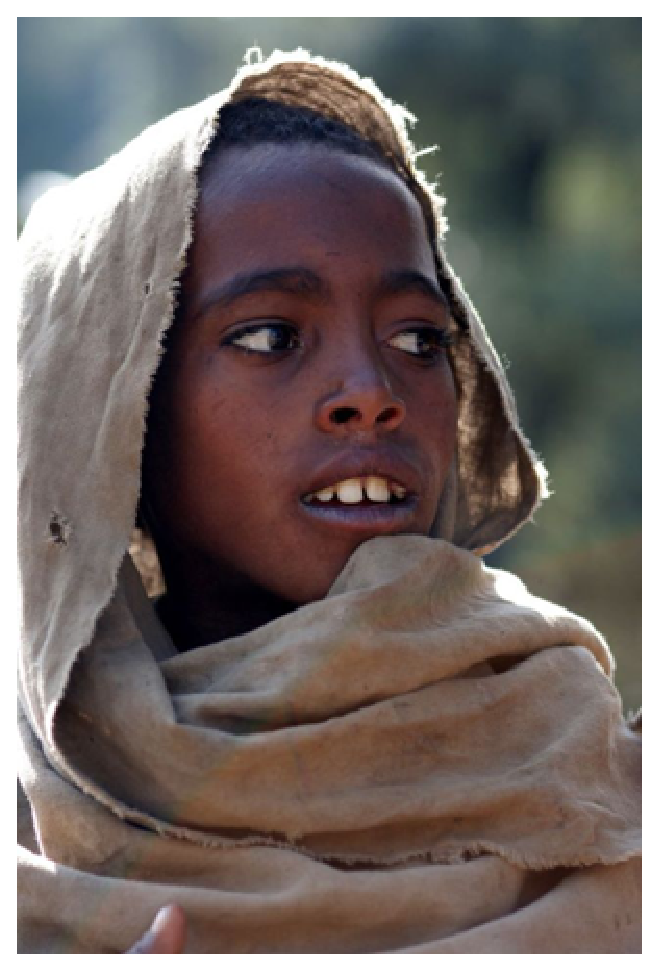
\includegraphics{etiopan.eps}\hspace{-0.13cm}
		\reflectbox{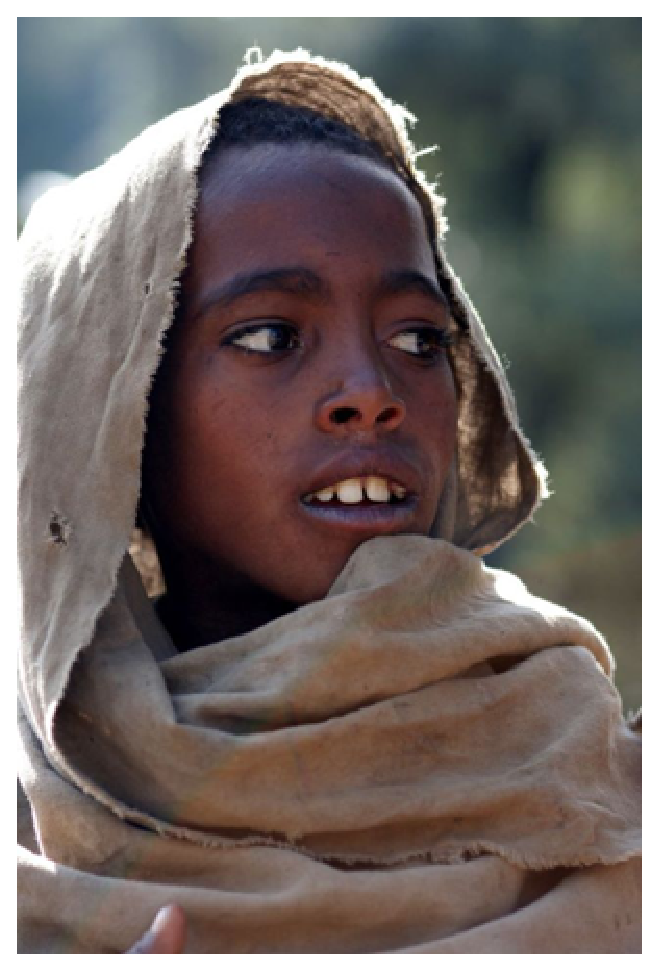
\includegraphics{etiopan.eps}}}
		\caption{Malý etiopánek a jeho bratříček}
		\label{etiopani}
	\end{center}

\end{figure}



\newpage

Rozdíl mezi vektorovým \ldots

\begin{figure}[h]

	\begin{center}
		\scalebox{0.4}{
\includegraphics{oniisan.eps}}
		\caption{Vektorový obrázek}
		\label{vektorovy}
	\end{center}

\end{figure}

\ldots a bitmapovým obrázkem

\begin{figure}[ht]

	\begin{center}
		\scalebox{0.6}{
\includegraphics{oniisan2.eps}}
		\caption{Bitmapový obrázek}
		\label{bitmapovy}
	\end{center}

\end{figure}

\noindent{se projeví například při zvětšení.}
\par Odkazy (nejen ty) na obrázky \ref{etiopani}, \ref{vektorovy} a \ref{bitmapovy}, na tabulky \ref{tabulka1} a \ref{tabulka2} a také na algoritmus \ref{algoritmus1} jsou udělány pomocí křížových odkazů. Pak je ovšem potřeba zdrojový soubor přeložit dvakrát.
\par Vektorové obrázky lze vytvořit i přímo v \LaTeX u, například pomocí prostředí \texttt{picture}. Všechny rozměry jsou uváděny v mm.

\end{document}